\subsection{Language Server}

VS-Code Plugins can be implemented in two ways: the first one is via the standard VS-CODE API and the second one is in form of a language server. Language servers follow a standard protocol to provide services for working with different programming languages and offer often used features such as go to definition. While this offers great portability and easy integration with other IDEs or tools that work with language server, the implementation as a language server was rejected in this project. \newline
The main reason is that the project extends an existing plugin, which was already built around the standard VS-CODE API. After a phase of research and writing a small prototype it was decided that rewriting the plugin as a language server was not a feasable in regard to the work needed to be done compared to the project scope. \newline
A second consideration when making this decision was that the usage of language servers in VS-CODE plugins is very sparse at the moment. The big language integrations like typescript or javascript do not implement their plugins as language servers, while the golang plugin offers experimental support at this time. The not wide spread usage in this environment was therefore another reason to not implement a language server.


Server here refers to the Language Server and not the DafnyServer. The later one is explictily written as DafnyServer.

\subsubsection{Communication Types}

\paragraph{Notification}

\paragraph{Request}

\paragraph{Commands}


\subsubsection{Communication overview}

\paragraph{Diagnostics Server ---> Client}

\textbf{sendDiagnostics}

\paragraph{Notification Server ---> Client}

\textbf{ERROR}

\textbf{WARNING}

\textbf{INFO}

\textbf{queueSize}

\textbf{serverStarted}

\textbf{activeVerifiyingDocument}

\textbf{verificationResult}

\textbf{hideStatusbar}

\textbf{changeServerStatus}

\textbf{ready}

\paragraph{Request Server ---> Client}

\textbf{dafnymissing}


\paragraph{Notification Client ---> Server}

\textbf{verify}

\paragraph{Request Client ---> Server}

\textbf{reset}

\textbf{compile}

\textbf{stop}


\paragraph{Commands Client}

\textbf{dafny.restartDafnyServer}

\textbf{dafny.installDafny}

\textbf{dafny.uninstallDafny}

\textbf{dafny.showReferences}

\textbf{dafny.editText}

\textbf{dafny.compile}

Shortcut: ctrl+shift+b or %⇧⌘B

\textbf{dafny.compileAndRun}

Shortcut: F5


\subsubsection{Startup process}
\begin{figure}[H]
	\centering
	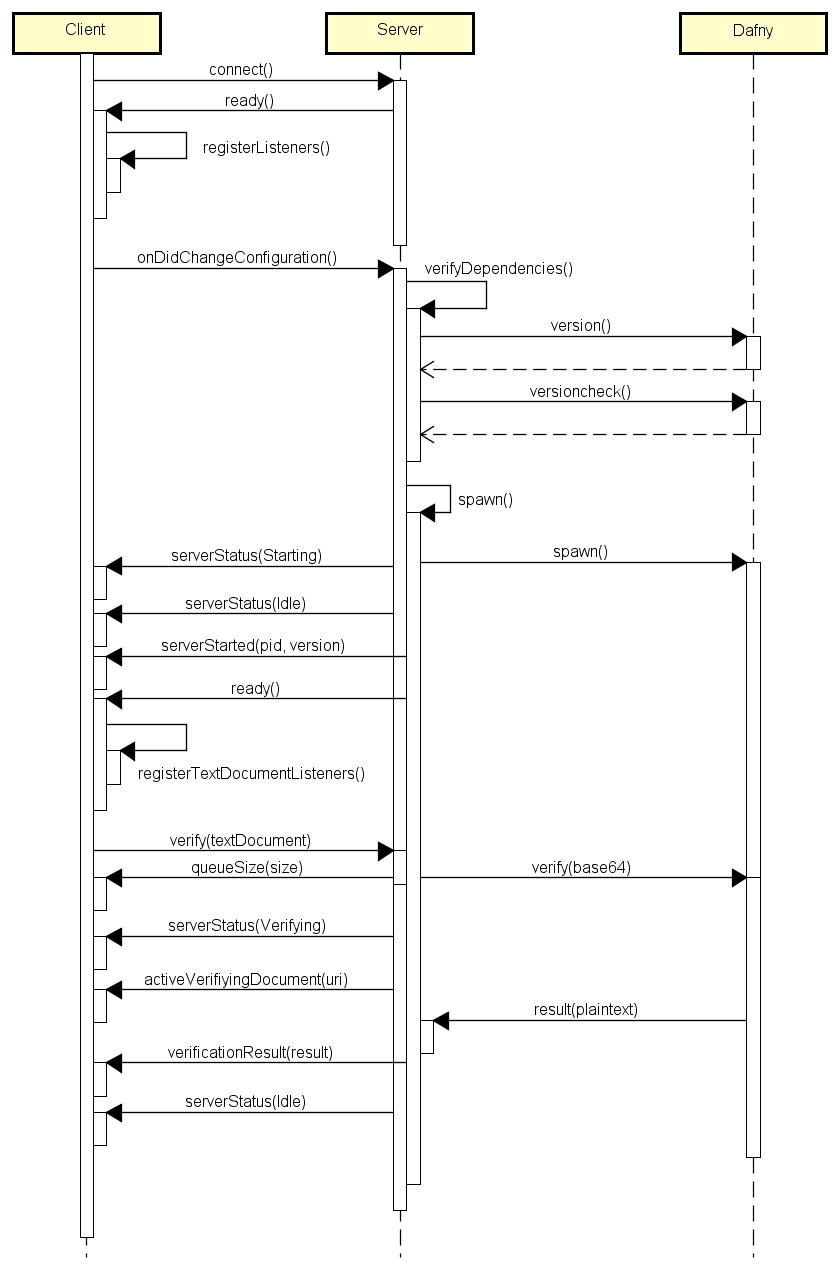
\includegraphics[width=1\textwidth]{img/DafnyStartupFull}
	\caption{DafnyServer startup}
	\label{fig:DafnyServer startup}
\end{figure}

\subsubsection{Not installed}
\begin{figure}[H]
	\centering
	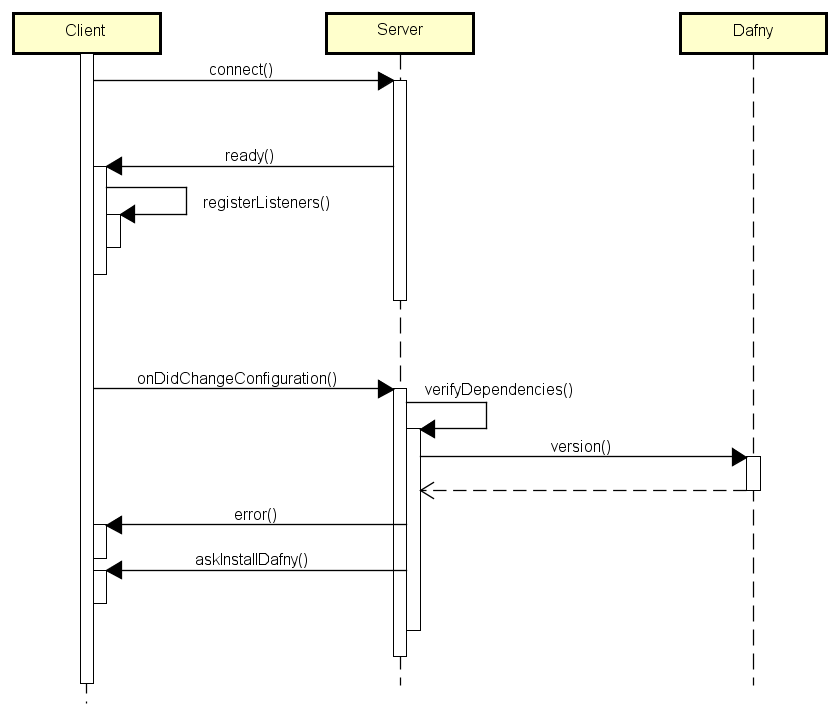
\includegraphics[width=1\textwidth]{img/DafnyNotInstalled}
	\caption{Dafny not installed}
	\label{fig:Dafny not installed}
\end{figure}

\subsubsection{Installation - Upgrade available}
\begin{figure}[H]
	\centering
	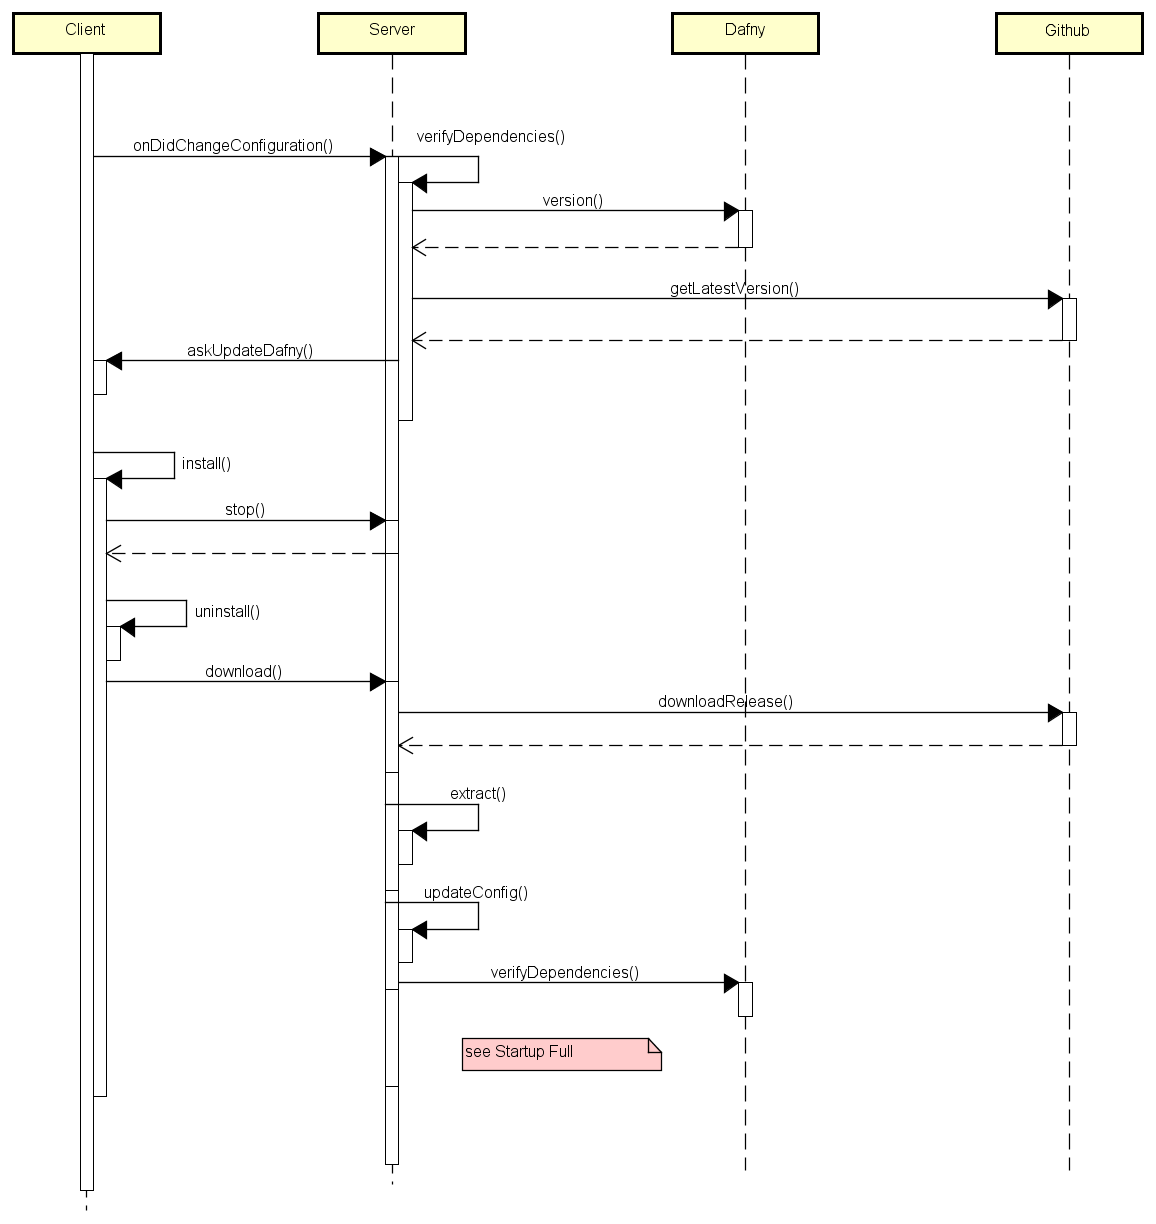
\includegraphics[width=1\textwidth]{img/DafnyVersionUpgrade}
	\caption{Version upgrade available}
	\label{fig:Version upgrade available}
\end{figure}



